\documentclass[a4paper,10pt]{article}
\usepackage[utf8x]{inputenc}
\usepackage{url}
\usepackage{amsmath}
\usepackage{graphicx}
\usepackage[pdftex,                %
    bookmarks         = true,%     % Signets
    bookmarksnumbered = true,%     % Signets num\'erot\'es
    pdfpagemode       = None,%     % Signets/vignettes ferm\'e \`a l'ouverture
    pdfstartview      = FitH,%     % La page prend toute la largeur
    pdfpagelayout     = SinglePage,% Vue par page
    colorlinks        = false,%     % Liens en couleur
    urlcolor          = magenta,%  % Couleur des liens externes
    pdfborder         = {0 0 0}%   % Style de bordure : ici, pas de bordure
    ]{hyperref}%                   % Utilisation de HyperTeX

\hypersetup {
colorlinks=false;
bookmarks=true;
pdftitle={IA pour robots voyageurs}
pdtauthor={Christophe Labedan}
pdfsubject={Ricochet Robots algorithm}
pdfcreator  = {PDFLaTeX}
pdfproducer = {PDFLaTeX}
}


% Title Page
\title{MAIA - IA POUR ROBOTS VOYAGEURS\\Responsable: Alexandre DUTECH}
\author{}
\date{}

\begin{document}
\maketitle

% \begin{abstract}
% \end{abstract}

\section*{Probl\'ematique de recherche :}
Planification de trajectoires complexes dans un environnement qui peut
n'être que partiellement connu. Ce sujet est aussi une initiation \`a
l'utilisation d'algorithme de recherche heuristique avec une
application dans le cadre des jeux.

\section*{Sujet :}
Le but du stage est de r\'ealiser une Intelligence Artificielle pour
r\'esoudre les probl\`emes des "Robots Voyageurs" (voir
\url{http://www.ricochetrobots.com/RR.html} pour y "jouer" en ligne).

Dans un premier temps, il s'agira d'impl\'ementer une m\'ethode de
recherche de type A*. La premi\`ere difficult\'e sera alors de valider la
ou les heuristiques utilis\'ees.

Dans un deuxi\`eme temps, l'environnement sera compliqu\'e par l'ajout
d'\'el\'ements apportant des incertitudes sur l'\'etat du monde. Les
algorithmes de planifications "classiques" et d\'eterministes seront alors
compar\'es \`a d'autres m\'ethodes comme par exemple : planification
probabilistes, algorithmes g\'en\'etiques, m\'ethodes de monte-carlo. Chaque
membre du bînome pourra s'attacher \`a la mise en oeuvre d'une de ces
m\'ethodes.

\section*{Ref. Biblio :}

\cite{AIMA} Artificial Intelligence: A Modern Approach. Stuart \&
Russel, Prentice Hall, 1995. Chap. 3.5 - Informed (Heuristic) Search
Strategies.

\newpage

\section{3 mars 2010}

\subsection{Rencontre}
\begin{itemize}
  \item[-]support: jeu Ricochet Robots (ou Randolph's Robots ou Rasender
Roboter)
  \item[-]A* est-il adapté à la résolution de ce problème ?
  \item[-]autres système(s) de résolution ?
\end{itemize}

\subsection{Recherche}

\begin{description}

  \item[Documentation]:
    \begin{itemize}
      \item[\cite{HMP}]Article étudiant certains algorithmes de résolution (parcours en largeur et en
    profondeur). Le problème est vu d'un point de vue cognition (étude sur une population).
      \item[\cite{NPC}]Article analysant la complexité du problème $\rightarrow$ NP-Complet.
    \end{itemize}

  \item[Idées]:
    \begin{itemize}
      \item[-]A* n'est pas bon: utilise une pondération des distances $\rightarrow$ pas de sens ici.
      \item[-]Apprentissage de la carte, que connaissent les robots ?
      \item[-]Algorithme génétique $\rightarrow$ construire une solution par ``mixage'' de solutions.
      \item[-]Arbres de décision $\rightarrow$ lourd.
    \end{itemize}

\end{description}

\section{11 mars 1010}
\subsection{Rencontre}

\begin{itemize}
  \item[-]A*: la pondération pourrait se faire par rapport au nombre de coût.
	    \\$longueur = g + h(s)$ où h est l'heuristique $\rightarrow$ \textbf{quelle heuristique ?}
  \item[-]Algorithme génétique: ``fitness function'' $\rightarrow$ attribuer une valeur à chaque solution pour pouvoir les comparer.
  \item[-]Apprentissage: quelles bases au départ, et comment généraliser ?
  \item[-]Recherche dirigée (ou heuristique) $\rightarrow$ propriétés de l'heuristique pour qu'elle soit utile ?
  \item[-]Force brute: pouvoir comparer l'efficacité avec d'autres solutions.
\end{itemize}

\vspace{1cm} Pour la prochaine fois:
\begin{itemize}
  \item[-]Thomas $\rightarrow$ A*
  \item[-]Jeremy $\rightarrow$ bruteforce
  \item[-]Christophe $\rightarrow$ algorithme génétique
\end{itemize}

\subsection{Recherche}
  \begin{itemize}
    \item[Thomas : ]
      \begin{itemize}
        \item[\dag]Impl\'ementation d'un programme permettant de mod\'eliser le probl\`eme.
        \item[\dag]Analyse de l'algorithme $A^*$ $\rightarrow$ probl\`eme pour trouver l'heuristique.
      \end{itemize}
    \item[Christophe : ]
      \begin{itemize}
        \item[\dag]Analyse des algorithmes g\'en\'etiques \cite{MOP} $\rightarrow$ probl\`eme pour trouver l'heuristique.
        \item[\dag]D\'ebut de recherche sur ``l'atteignabilit\'e de la cible''.
      \end{itemize}

    \item[$\Rightarrow$] Tests du programme avec des d\'eplacements al\'eatoires $\rightarrow$ certaines cases sont plus souvent visit\'ees que d'autres, certaines ne le sont jamais.
  \end{itemize}



\section{25 mars 2010}
\subsection{Rencontre}
\par Pr\'esentation des r\'esultats de nos recherches, discussion pour essayer de trouver une piste sur comment trouver de bonnes heuristiques.
\par Par rapport \`a l'atteignabilit\'e, il faut essayer de formaliser ce dont il s'agit, montrer si cela permet effectivement de trouver des solutions, et si oui, sont-elles optimales ? Quelle est la couverture de l'algorithme ?
\par Au niveau de la recherche par force brute, l'algorithme n'est pas encore au point, il faudra notamment \'etudier les types de parcours dans les arbres existants.
\par Prochaine fois : s\'eminaire sur la synth\`ese d'images.

\newpage

\bibliographystyle{unsrt}
\bibliography{biblio}


\clearpage
\appendix
\section{Algorithmes \'evolutionnaires - cas des algorithmes g\'en\'etiques}
\subsection{Terminologie \cite{MOP}}

\begin{description}
  \item[Individu]: Une solution au probl\`eme pos\'e; elle peut \^etre plus ou moins performante.
  \item[Population]: Ensemble des individus trait\'es simultan\'ement par l'algorithme \'evolutionnaire.
  \item[G\'en\'erations]: It\'erations durant lesquelles \'evolue la population, jusqu'\`a ce qu'un crit\`ere d'arr\^et soit v\'erifi\'e.
  \item[Parent]: Individu soumis \`a un op\'erateur.
  \item[Enfant]: Individus r\'esultant de l'application d'un op\'erateur.
\end{description}


\subsection{Principe}
Le principe d'un algorithme g\'en\'etique est d'appliquer une variation (mutation et/ou croisement) sur un ou plusieurs individus. Dans le cas d'une mutation, un individu est modifi\'e al\'eatoirement, la taille de la population n'est donc pas modifi\'ee. Un croisement s'applique sur n individus de la population. Il s'agit de combiner suivant certains crit\`eres ces individus.\\
Pour pouvoir appliquer une variation, il est n\'ecessaire de d\'efinir un codage qui repr\'esentera n'importe quel individu d'une population. Cela permet de r\'ealiser des coupures ou des \'echanges par exemple sur les individus.\\

La qualit\'e d'un individu peut d\'eterminer son taux d'utilisation pour la reproduction. Pour la d\'eterminer, il faut d\'efinir une fonction de performance (\textit{fitness function}) affectant \`a chaque individu une valeur de performance. L'inconv\'enient d'une telle fonction est qu'il faut la recalculer \`a chaque it\'eration pour mettre \`a jour la population.
Plusieurs strat\'egies de s\'elections peuvent \^etre utilis\'ees: 
\begin{itemize}
  \item[-] la s\'election d\'eterministe : seuls les n meilleurs individus sont s\'electionn\'es,
  \item[-] les tournois stochastiques : les n meilleurs individus sont choisis chacun avec une probabilit\'e comprise entre 0,5 et 1.
  \item[-] les tournois d\'eterministes : la s\'election est al\'eatoire.
  \item[-] le remplacement de g\'en\'eration : on ne garde que les enfants
\end{itemize}

\begin{figure}
  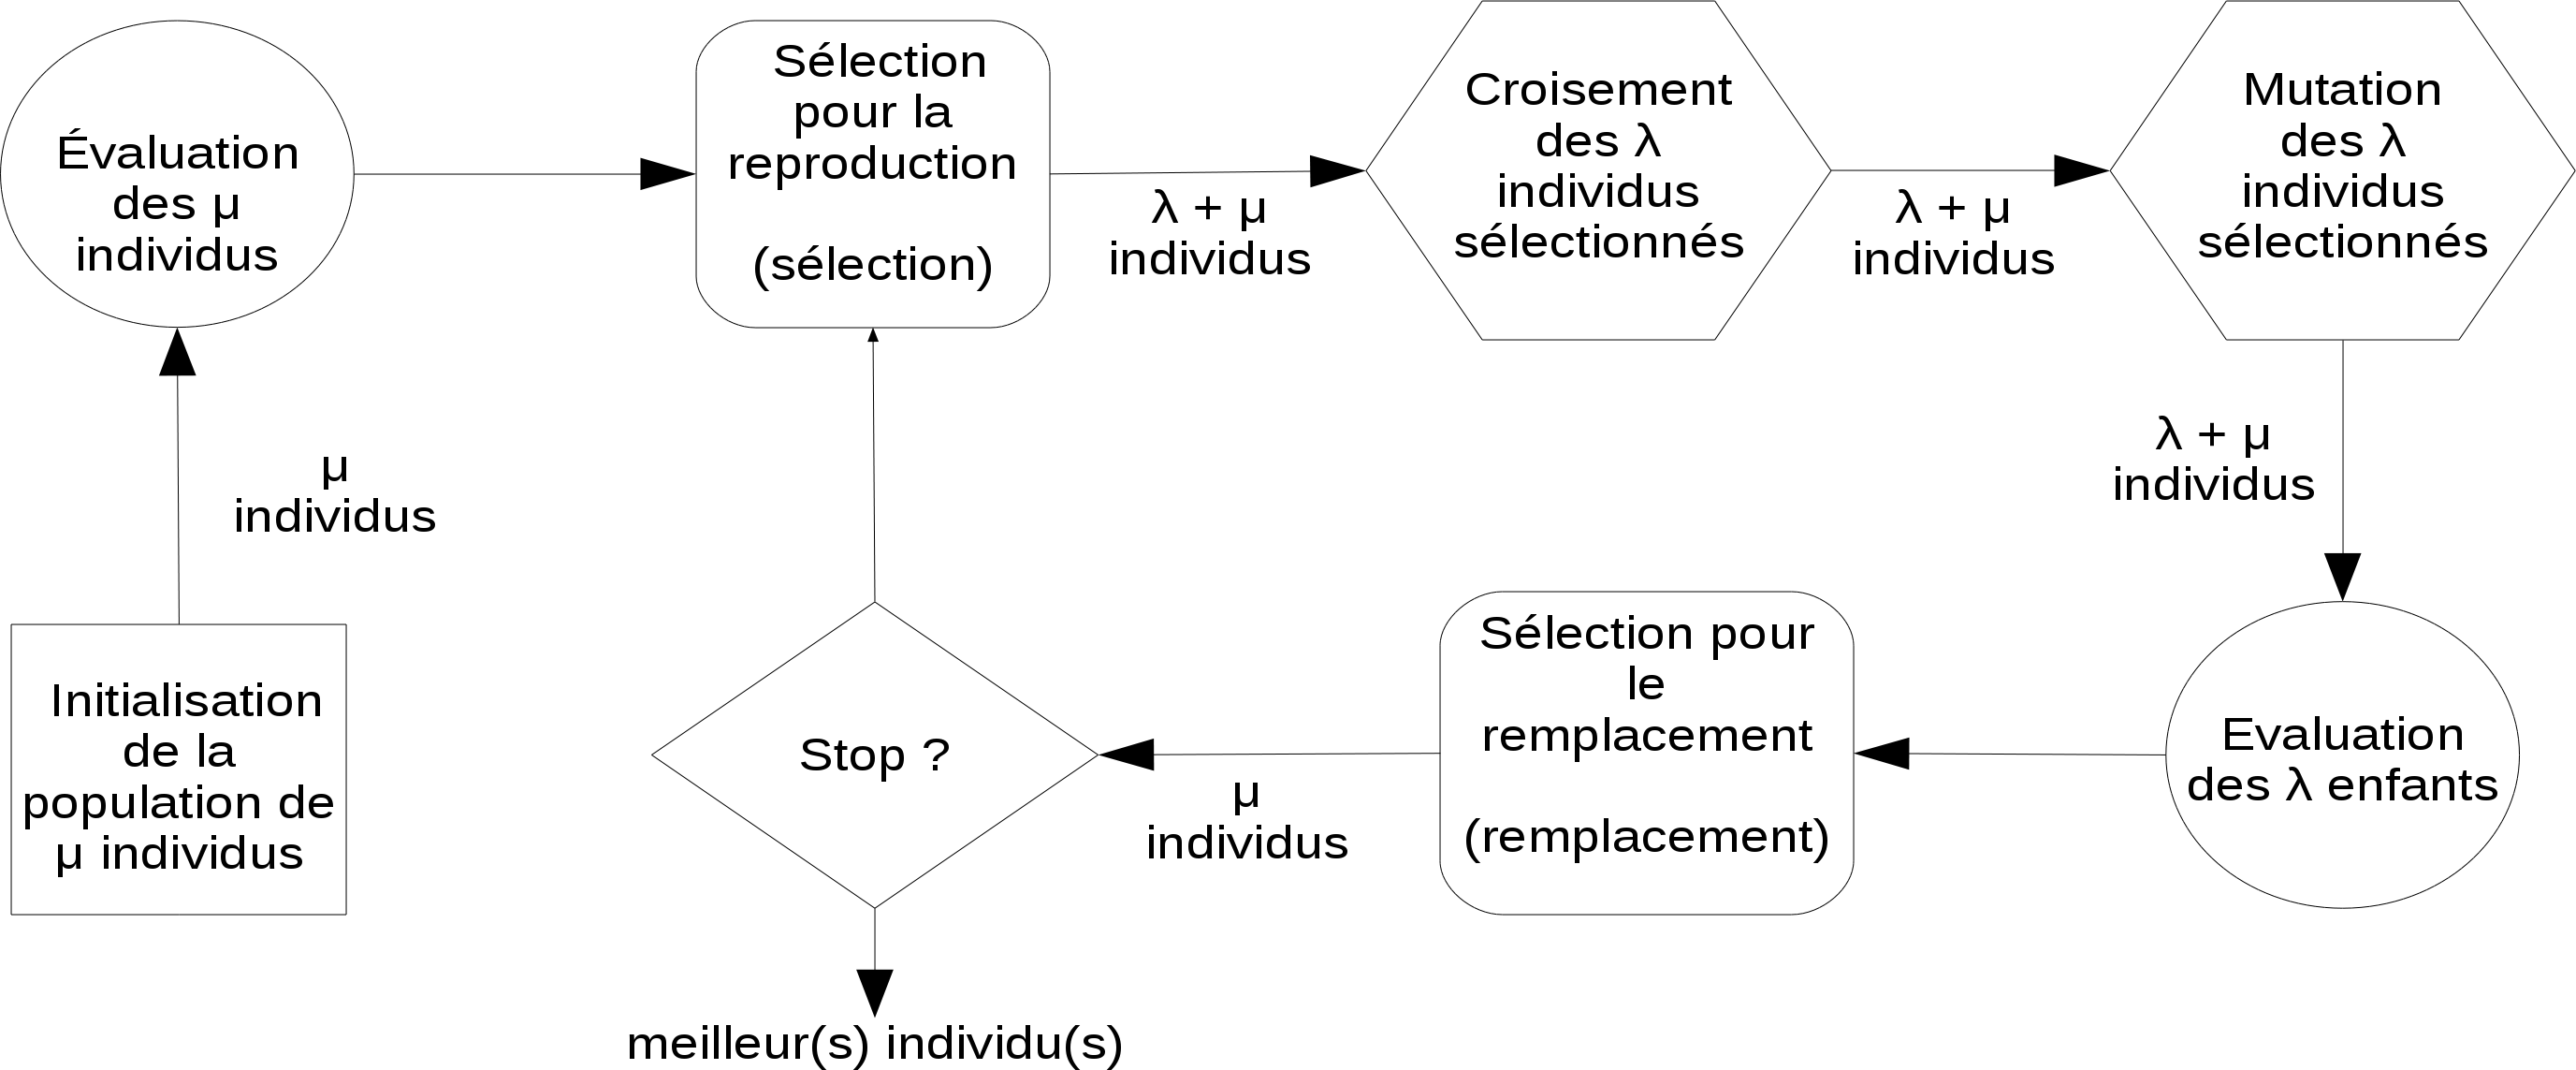
\includegraphics[width=\linewidth]{img/cycle.png}
  \caption{L'algorithme \'evolutionnaire g\'en\'erique \cite{MOP}}
\end{figure}

Le probl\`eme ``Ricochet Robots'' peut \^etre mod\'elis\'e par une matrice d'adjacences. Un individu sera rep\'esent\'e par un vecteur contenant une liste de sommets adjacents. Apr\`es avoir construit la population, un individu est choisit au hasard, et supprim\'e des autres listes afin de ne pas faire demi tour. Cet individu est ensuite crois\'e avec un autre selon une strat\'egie \`a d\'efinir. On recommence ce processus tant qu'un chemin valide n'a pas \'et\'e trouv\'e (chemin du robot \`a sa cible).\\
Il est \`a noter que dans ce probl\`eme, plusieurs populations sont envisageables (une par robot). Il faut donc d\'efinir les interactions entre celles-ci. De plus, il faut d\'efinir une ``fitness function''. Ici, elle devra prendre en compte la taille du vecteur (le nombre de coups effectu\'es), et le fait que la cible appartient ou non \`a la liste.


\end{document}          
